\documentclass[aspectratio=1610]{beamer}

% Theme choice
\usetheme{focus}

\definecolor{main}{RGB}{0, 80, 60}
\definecolor{background}{RGB}{255, 255, 255}

\newcommand{\vuwlogo}{%
    \begin{tikzpicture}[remember picture,overlay]
    \node[anchor=north east,yshift=3.5pt,xshift=0pt] at (current page.north east) {\includegraphics[height=0.95cm]{figures/vuw.png}};
    \node[anchor=north east,yshift=3.5pt,xshift=-70pt] at (current page.north east) {\includegraphics[height=0.95cm]{figures/evostar2025.png}};
    \end{tikzpicture}%
}

\setbeamertemplate{navigation symbols}{}
\setbeamertemplate{footline}[frame number]

% Packages
\usepackage{amsmath}
\usepackage{amssymb}
\usepackage{graphicx}
\usepackage{booktabs}
\usepackage{algorithm}
\usepackage{algpseudocode}
\usepackage{tikz}
\usetikzlibrary{shapes,arrows,positioning}

% Title information
\title[RAG-SR]{RAG-SR: Retrieval-Augmented Generation for Neural Symbolic Regression}
\author[Zhang et al.]{Hengzhe Zhang, Qi Chen, Bing Xue, Wolfgang Banzhaf, Mengjie Zhang}
\institute[VUW \& MSU]{
    School of Engineering and Computer Science, Victoria University of Wellington\\
    Department of Computer Science and Engineering, Michigan State University
}
\date{ICLR 2025 (Spotlight)}

\begin{document}

% Title slide
    \begin{frame}
        \titlepage
    \end{frame}

% Outline
    \begin{frame}{Outline}
        \tableofcontents
    \end{frame}


    \section{Introduction}

    \begin{frame}{Symbolic Regression}
        \begin{itemize}
            \item \textbf{Symbolic Regression (SR)} discovers mathematical expressions that best describe a dataset
            \item Automatically determines both the \textbf{structure} $f$ and \textbf{parameters} $\theta$ of the model
            \item Offers both \textbf{high accuracy} and \textbf{interpretability}
            \item Applications: physics, biology, finance, scientific discovery
        \end{itemize}

        \vspace{0.3cm}

        \textbf{Mathematical Definition:}
        \begin{align}
        (f^*, \theta^*)
            = \underset{f \in \mathcal{F}, \theta}{\text{argmin}} \sum_{i=1}^n \mathcal{L}(f(x_i, \theta), y_i)
        \end{align}
    \end{frame}

    \begin{frame}{Problem Formulation: Feature Construction Approach}
        \begin{itemize}
            \item Generate a set of symbolic trees/features $\Phi = \{\phi_1, \ldots, \phi_m\}$ from dataset $(X, Y)$
            \item Enhance interpretable model $\mathcal{M}$ (e.g., linear regression)
            \item Objective: Minimize loss function
        \end{itemize}

        \begin{equation}
            \mathcal{L}(\Phi; X, Y) = \frac{1}{N} \sum_{i=1}^{N} \ell\left(\mathcal{M}\left(\phi_1(X_i), \ldots, \phi_m(X_i)\right), Y_i\right)
        \end{equation}

        \vspace{0.3cm}
        \textbf{Advantages:}
        \begin{itemize}
            \item Effective for complex real-world problems
            \item Multiple weak features can collectively work well
        \end{itemize}
    \end{frame}


    \begin{frame}{Limitations of Current Approaches: Pre-trained Models}

        \begin{center}
            \textbf{Pre-trained Models}
            \begin{itemize}
                \item Limited to seen functions
                \item Struggles with new variables
                \item Requires large pre-training
            \end{itemize}
            \includegraphics[width=0.7\textwidth]{figs/E2E.png}
        \end{center}
    \end{frame}

    \begin{frame}{Limitations of Current Approaches: Reinforcement Learning}

        \begin{center}
            \textbf{Reinforcement Learning}
            \begin{itemize}
                \item Low sample efficiency
                \item Limited feedback
                \item Slow convergence
            \end{itemize}
            \includegraphics[width=0.7\textwidth]{figs/DSR.png}
        \end{center}
    \end{frame}

    \begin{frame}{Limitations of Current Approaches: Sparse Supervised Learning}

        \begin{center}
            \textbf{Sparse Supervised Learning}
            \begin{itemize}
                \item Relies on heuristic pruning
                \item Produces potentially large solutions
                \item Requires differentiable activation functions
            \end{itemize}
            \includegraphics[width=0.7\textwidth]{figs/EQL.png}
        \end{center}
    \end{frame}


    \begin{frame}{Related Work}
        \begin{columns}
            \begin{column}{0.48\textwidth}
                \textbf{Neural Symbolic Regression}
                \begin{itemize}
                    \item Pre-trained models (DSR, E2E) struggle with unseen functions/variables
                    \item RL approaches have low sample efficiency
                    \item Sparse supervised learning requires differentiable activation functions
                \end{itemize}
            \end{column}
            \begin{column}{0.48\textwidth}
                \textbf{Evolutionary Symbolic Regression}
                \begin{itemize}
                    \item Traditional GP lacks search effectiveness
                    \item Semantic GP is effective but relies solely on existing building blocks
                    \item Limited knowledge retention during evolution
                \end{itemize}
            \end{column}
        \end{columns}
    \end{frame}


    \begin{frame}{Key Insight: Guiding Neural Generation with Good Solutions}
        \begin{alertblock}{Key Insight}
            \textbf{From LM perspective:}
            \begin{itemize}
                \item Using neural networks to directly improve solutions leads to hallucination
                \item Better approach: Show the model potentially good improvements and ask it to generate better ones
            \end{itemize}

            \textbf{From EA perspective:}
            \begin{itemize}
                \item Instead of asking "give me a good mutation," we show examples of good mutations and say "a good mutation is like this, give me a better one"
            \end{itemize}

            \textbf{When using LLMs like ChatGPT:}
            \begin{itemize}
                \item Don't ask: "The current program only does B, but I want it to do A"
                \item Instead ask: "The current program only does B, I want it to do A, and I think a potential direction is..."
            \end{itemize}
        \end{alertblock}
    \end{frame}


    \begin{frame}{RAG-SR: A Novel Semantic-to-Symbolic Learning Framework}
        \textbf{Our Approach:} Integrating evolutionary feature construction with neural networks through online learning

        \begin{itemize}
            \item \textbf{Semantic Descent:} Adaptively generates symbolic trees aligned with desired semantics in real-time through online supervised learning

            \item \textbf{Retrieval-Augmented Generation:} Mitigates hallucinations by leveraging symbolic expressions in a library

            \item \textbf{Masked Contrastive Learning:} Captures semantically equivalent but syntactically different symbolic expressions

            \item \textbf{Scale-invariant Data Augmentation and Double Query Strategy:} Improves robustness to linear regression
        \end{itemize}
    \end{frame}


    \section{Methodology}

    \begin{frame}{RAG-SR: Solution Initialization \& Evaluation}
        \begin{columns}
            \begin{column}{0.5\textwidth}
                \textbf{Step 1: Solution Initialization}
                \begin{itemize}
                    \item Random symbolic trees using ramped half-and-half
                \end{itemize}

                \vspace{0.3cm}
                \textbf{Step 2: Solution Evaluation}
                \begin{itemize}
                    \item Features evaluated via ridge regression with LOOCV
                \end{itemize}
            \end{column}
            \begin{column}{0.5\textwidth}
                \includegraphics[width=1.0\textwidth]{figs/Workflow.pdf}
            \end{column}
        \end{columns}
    \end{frame}

    \begin{frame}{RAG-SR: Semantic Library Construction}
        \begin{columns}
            \begin{column}{0.5\textwidth}
                \textbf{Step 3: Semantic Library Construction}
                \begin{itemize}
                    \item \textbf{Retrieval Library:} FIFO queue with KD-Tree for efficient retrieval
                    \begin{itemize}
                        \item Semantics are normalized before storing because feature construction is insensitive to scale
                    \end{itemize}
                    \item \textbf{Neural Semantic Library:} Trained using pairs from retrieval library
                \end{itemize}
            \end{column}
            \begin{column}{0.5\textwidth}
                \includegraphics[width=1.0\textwidth]{figs/Workflow.pdf}
            \end{column}
        \end{columns}
    \end{frame}

    \begin{frame}{RAG-SR: Solution Selection Process}
        \begin{columns}
            \begin{column}{0.5\textwidth}
                \textbf{Step 4: Solution Selection}
                \begin{itemize}
                    \item Lexicase selection to select promising parents
                \end{itemize}
            \end{column}
            \begin{column}{0.5\textwidth}
                \includegraphics[width=1.0\textwidth]{figs/Workflow.pdf}
            \end{column}
        \end{columns}
    \end{frame}

    \begin{frame}{RAG-SR: Solution Generation}
        \begin{columns}
            \begin{column}{0.5\textwidth}
                \textbf{Step 5: Solution Generation}
                \begin{itemize}
                    \item \textbf{Semantic Descent:} Local search to improve solutions
                    \item \textbf{Evolutionary Search:} Global exploration with GP operators
                \end{itemize}
            \end{column}
            \begin{column}{0.5\textwidth}
                \includegraphics[width=1.0\textwidth]{figs/Workflow.pdf}
            \end{column}
        \end{columns}
    \end{frame}

    \begin{frame}{RAG-SR: Archive Maintenance}
        \begin{columns}
            \begin{column}{0.5\textwidth}
                \textbf{Step 6: Archive Maintenance}
                \begin{itemize}
                    \item Store best-performing solution
                \end{itemize}
            \end{column}
            \begin{column}{0.5\textwidth}
                \includegraphics[width=1.0\textwidth]{figs/Workflow.pdf}
            \end{column}
        \end{columns}
    \end{frame}

    \begin{frame}{Semantic Descent: Overview}
        % 图片放在上方
        \begin{center}
            \includegraphics[width=0.75\textwidth, trim=8pt 8pt 8pt 8pt, clip]{figs/Motivation.pdf}
        \end{center}

        % 文字放在下方
        \textbf{Key Principle:}
        \begin{itemize}
            \item Iterative optimization replacing suboptimal features while maintaining a constant feature count
        \end{itemize}
    \end{frame}

    \begin{frame}{Semantic Descent: Step 1-2}
        % 图片放在上方
        \begin{center}
            \includegraphics[width=0.75\textwidth, trim=8pt 8pt 8pt 8pt, clip]{figs/Motivation.pdf}
        \end{center}

        % 文字放在下方
        \textbf{For each tree $\phi_i$ in solution $\{\phi_1, \ldots, \phi_m\}$:}
        \begin{enumerate}
            \item Temporarily remove contribution of $\phi_i$:\\
            $\Phi^{temp}(X) = \Phi(X) - \beta_i \phi_i(X)$
            \item Compute residual $R = Y - \Phi^{temp}(X)$
        \end{enumerate}
    \end{frame}
    \begin{frame}{Semantic Descent: Step 3}
        % 图片放在上方
        \begin{center}
            \includegraphics[width=0.75\textwidth, trim=8pt 8pt 8pt 8pt, clip]{figs/Motivation.pdf}
        \end{center}

        % 文字放在下方
        \textbf{Generate a new tree to fill this gap using:}
        \begin{itemize}
            \item Neural generation with probability $P_{neural}$: "Here's a pattern that worked before, generate something better"
            \item Retrieval from semantic library with probability $1-P_{neural}$: "Find the best matching pattern we've seen before"
        \end{itemize}
    \end{frame}

    \begin{frame}{Semantic Descent: Step 4}
        % 图片放在上方
        \begin{center}
            \includegraphics[width=0.75\textwidth, trim=8pt 8pt 8pt 8pt, clip]{figs/Motivation.pdf}
        \end{center}

        % 文字放在下方
        \textbf{Final Step:}
        \begin{itemize}
            \item Accept new tree if it reduces error for Retrieval, directly accept if Neural generation
            \item Continue process iteratively for all trees in the solution
        \end{itemize}
    \end{frame}

    \begin{frame}{Retrieval-Augmented Generation}
        % 图片在上方
        \begin{center}
            \includegraphics[width=0.7\textwidth]{figs/NN.pdf}
        \end{center}

        % 文字在下方
        \textbf{Challenge:} Language model can always generate something, but may be irrelevant to the given task

        \textbf{Key Idea:} Retrieval-augmented generation to reduce hallucination

        \begin{itemize}
            \item \textbf{Data Collection:} Store evaluated subtrees and semantics in a library
            \item \textbf{Network Training:} Map semantics to symbolic expressions
            \item \textbf{Retrieval:} Provide context from promising expressions
        \end{itemize}
    \end{frame}

    \begin{frame}{Neural Network Architecture}
        % 图片在上方
        \begin{center}
            \includegraphics[width=0.7\textwidth]{figs/NN.pdf}
        \end{center}

        % 文字在下方
        \begin{itemize}
            \item \textbf{MLP with Residual Connections:} Processes desired semantics $R$
            \item \textbf{Transformer Encoder:} Processes nearest symbolic tree $\hat{\phi}$
            \item \textbf{Transformer Decoder:} Generates sequence of tokens for new tree
            \item \textbf{Output:} Valid symbolic tree $\phi$ with semantics aligned to $R$
        \end{itemize}
    \end{frame}



    \begin{frame}{Loss Function}
        \textbf{Dual-objective loss function:}

        \begin{equation}
            \mathcal{L} = \mathcal{L}_{\text{cross-entropy}} + \lambda \cdot \mathcal{L}_{\text{InfoNCE}}
        \end{equation}

        \textbf{Cross-Entropy Loss:} Traditional objective for sequence generation

        \textbf{InfoNCE Loss:} Contrastive learning to capture semantic equivalence
    \end{frame}


    \begin{frame}{Masked Contrastive Loss}
        \textbf{Objective:} Align embeddings from intention encoding and retrieval-augmented encoding

        \vspace{0.2cm}
        \textbf{Process:}
        \begin{itemize}
            \item Nearest semantics $\hat{\phi}(X) \in \mathbb{R}^{B \times N}$ → MLP → $\mathbf{F}_{\text{nearest}} \in \mathbb{R}^{B \times K}$
            \item Symbolic embedding $\mathbf{H}_{\text{Transformer}} \in \mathbb{R}^{B \times L \times D}$ → Average → $\mathbf{H}_{\text{avg}} \in \mathbb{R}^{B \times D}$
        \end{itemize}

        \vspace{0.2cm}
        \textbf{InfoNCE Loss with Masking:}
        \begin{equation}
            \mathcal{L}_{\text{InfoNCE}} = - \frac{1}{B} \sum_{i=1}^{B} \log \frac{\exp\left(\text{sim}(\mathbf{F}_{\text{nearest}}[i], \mathbf{H}_{\text{avg}}[i]) / \tau\right)}{\sum_{j=1}^{B} \exp\left(\text{sim}(\mathbf{F}_{\text{nearest}}[i], \mathbf{H}_{\text{avg}}[j]) \cdot \text{mask} / \tau\right)}
        \end{equation}


    \end{frame}


    \begin{frame}{Effect of Contrastive Learning}
        \begin{columns}
            \begin{column}{0.55\textwidth}
                \begin{figure}
                    \centering
                    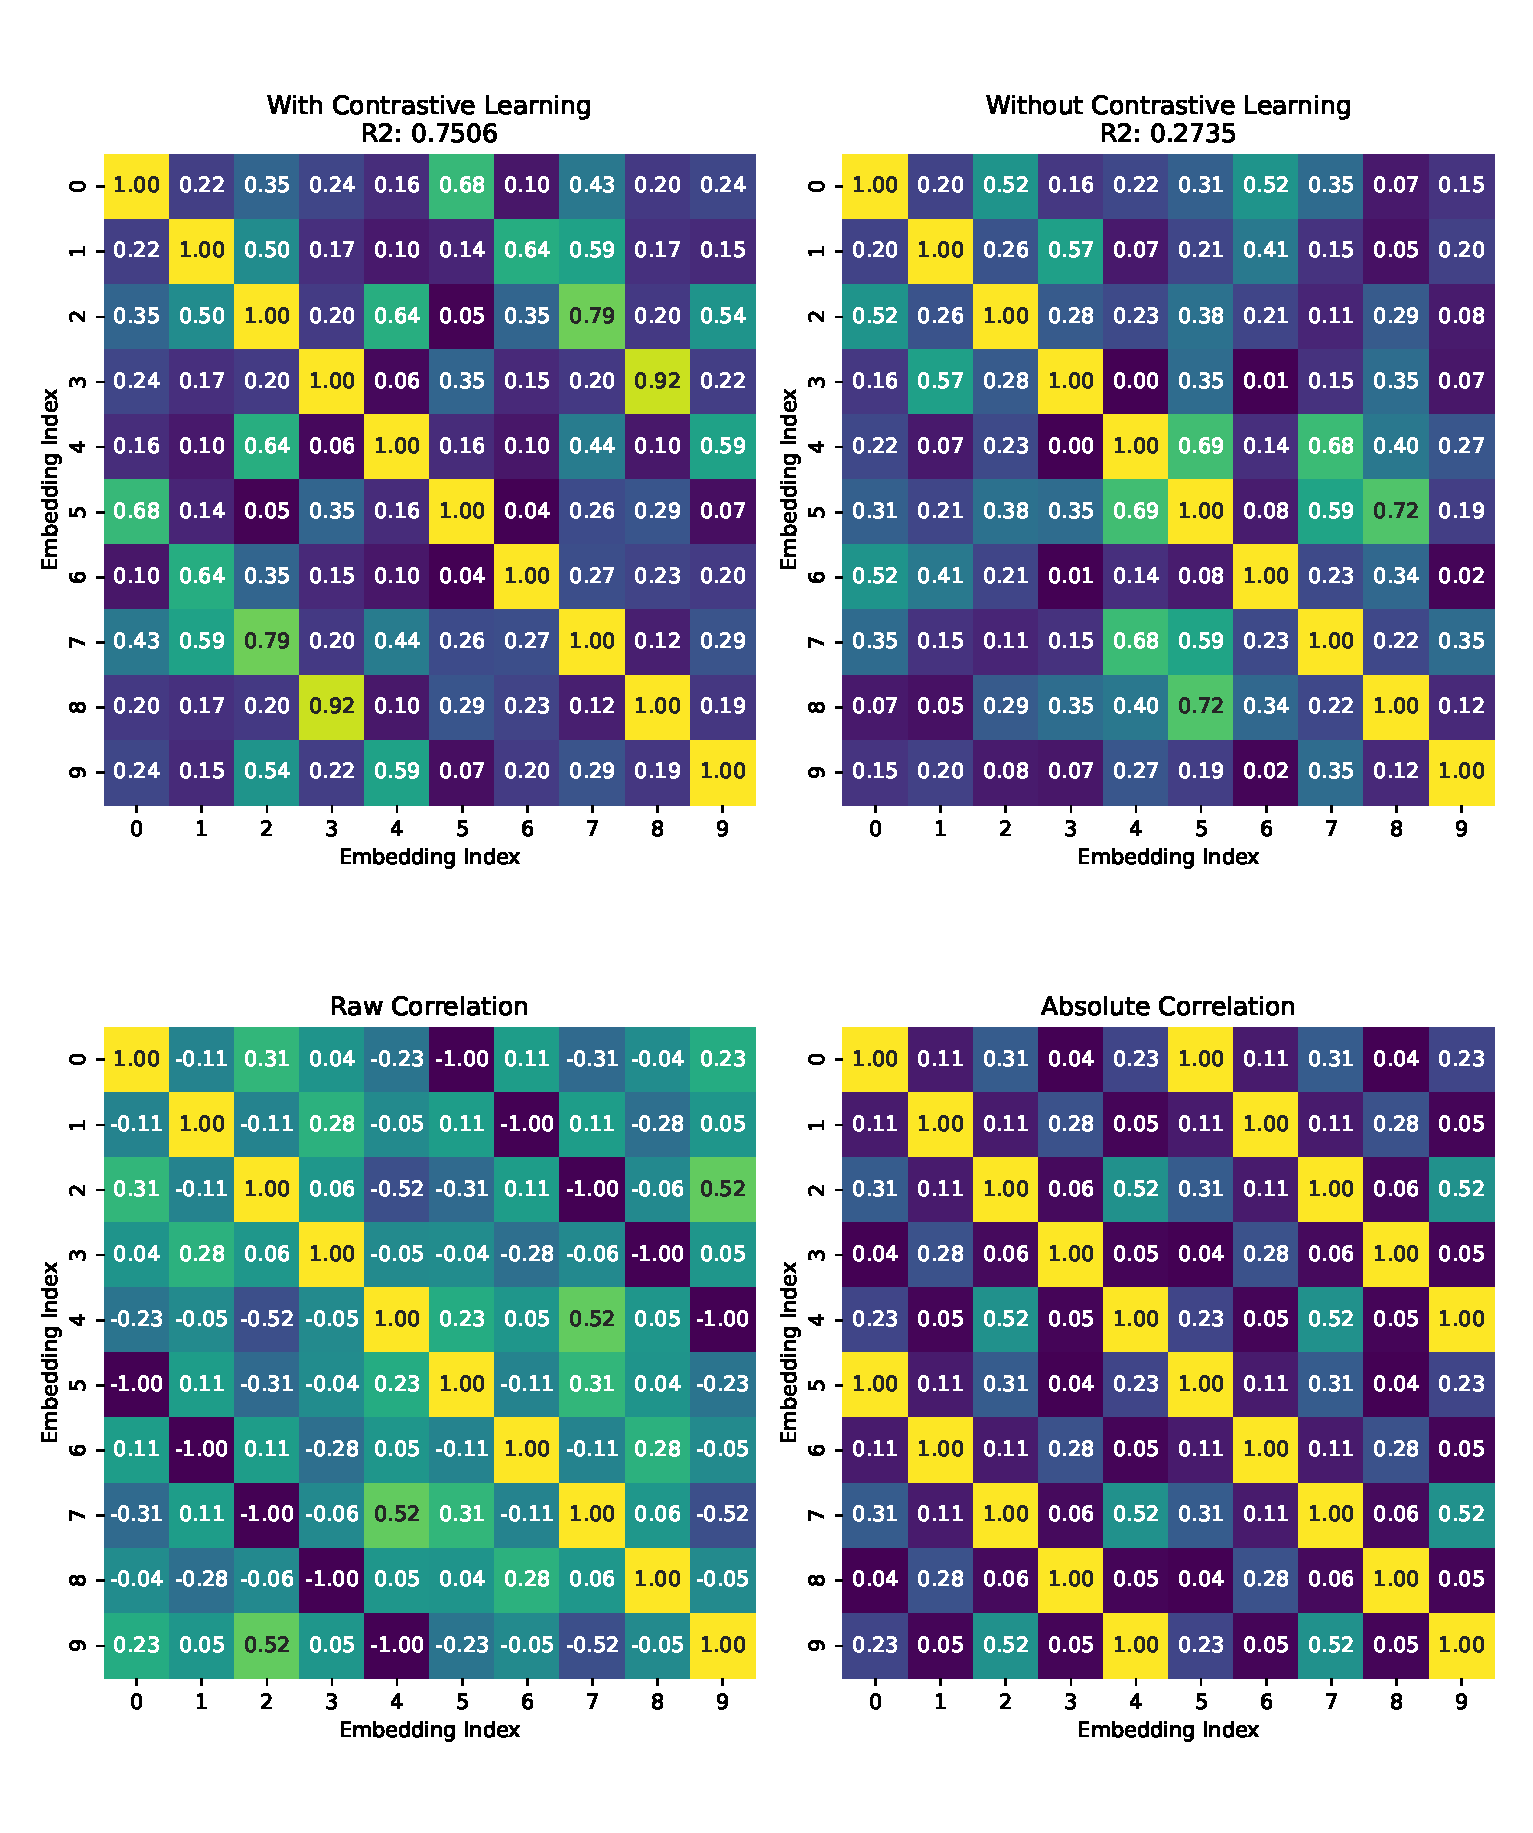
\includegraphics[height=0.8\textheight]{figs/data_augmentation_heatmap.eps}
                \end{figure}
            \end{column}

            \begin{column}{0.45\textwidth}
                \textbf{Mask Strategy:}
                \begin{itemize}
                    \item Mask matrix eliminates false negatives (cosine similarity > 0.99)
                    \item Prevents penalizing semantically similar expressions
                    \item Improves discrimination between truly different expressions
                \end{itemize}

                \textbf{Key Findings:}
                \vspace{0.3cm}
                \begin{itemize}
                    \item Captures different expressions with the same semantics as equivalent
                    \vspace{0.2cm}
                    \item Without it: different embeddings for equivalent semantics
                    \vspace{0.2cm}
                \end{itemize}
            \end{column}
        \end{columns}
    \end{frame}

    \begin{frame}{Data Augmentation \& Double Query}
        \textbf{Sign-invariant Property:} In linear regression, sign of coefficients is automatically adjusted

        \textbf{Data Augmentation:} Include both the original feature pairs $(\psi, \psi(X))$ and their negations $(\psi, -\psi(X))$
        \begin{equation}
            \mathcal{T} \gets \mathcal{T} \cup \{(\psi, -\psi(X)) \mid (\psi, \psi(X)) \in \mathcal{T}\}
        \end{equation}

        \textbf{Double Query:}
        \begin{itemize}
            \item Query the neural network with both the desired semantics $R$ and its negation $-R$
            \item Generate candidate trees $\phi$ and $\phi'$
            \item Select tree with highest probability
        \end{itemize}

    \end{frame}


    \section{Experiments}

    \begin{frame}{Experimental Setup}
        \textbf{Datasets:}
        \begin{itemize}
            \item 120 black-box datasets from PMLB benchmark
            \item 119 Feynman equations and 14 Strogatz datasets
        \end{itemize}

        \textbf{Evaluation Protocol:}
        \begin{itemize}
            \item 75:25 train-test split
            \item 10 repetitions for robustness
            \item $R^2$ score on test set as metric
            \item Min-max scaling of input features
        \end{itemize}

        \textbf{Configuration:}
        \begin{itemize}
            \item Population size: 200
            \item Generations: 100
            \item Solutions of 10 trees each
            \item $P_{neural} = 0.1$
        \end{itemize}
    \end{frame}

    \begin{frame}{Component Evaluation: Edit Distance}
        \begin{center}
            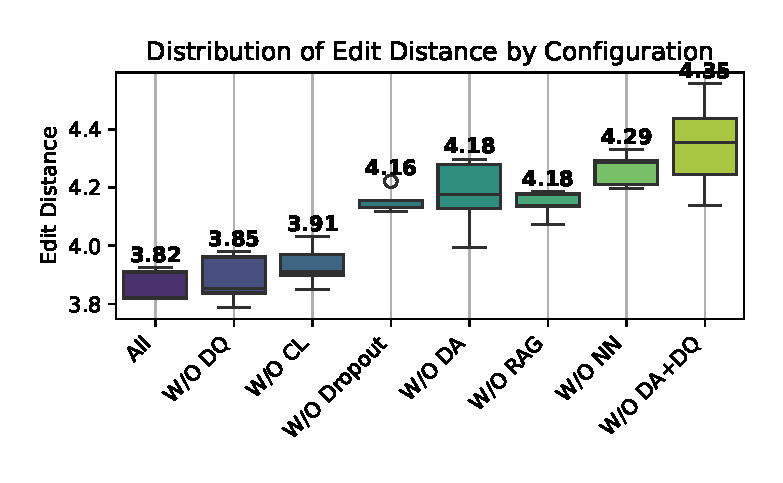
\includegraphics[width=0.6\textwidth]{figs/ablation_study_accuracy_10.eps}
        \end{center}

        \textbf{Observations:}
        \begin{itemize}
            \item Neural generation outperforms simple retrieval (W/O NN)
            \item All components together achieve lowest edit distance
            \item RAG has most significant impact, followed by data augmentation
            \item Dropout, contrastive learning, and double query show moderate benefits
        \end{itemize}
    \end{frame}

    \begin{frame}{Component Evaluation: Running Time}
        \begin{center}
            \includegraphics[width=0.6\textwidth]{figs/ablation_study_time_10.eps}
        \end{center}

        \textbf{Observations:}
        \begin{itemize}
            \item RAG moderately increases running time
            \item Removing DA and DQ reduces time but sacrifices accuracy
            \item Trade-off between computational cost and performance
            \item Acceptable overhead given accuracy improvements
        \end{itemize}
    \end{frame}

    \begin{frame}{Generated Trees Examples}
        \begin{table}
            \centering
            \footnotesize
            \begin{tabular}{cc}
                \toprule
                RAG-NN Generated Tree (Distance) & Simple NN Generated Tree (Distance) \\
                \midrule
                Sin(Sin(ARG3)) (0)               & Cos(Cos(Cos(ARG9))) (4)             \\
                AQ(ARG7, ARG8) (0)               & Log(Max(ARG7, ARG7)) (3)            \\
                Max(ARG1, ARG8) (0)              & Subtract(ARG1, ARG1) (2)            \\
                Sqrt(Sqrt(ARG2)) (0)             & Log(Log(ARG2)) (2)                  \\
                Subtract(ARG6, ARG7) (0)         & Max(ARG7, ARG7) (2)                 \\
                \bottomrule
            \end{tabular}
        \end{table}

        \begin{table}
            \centering
            \footnotesize
            \begin{tabular}{cc}
                \toprule
                Retrieval Tree (Distance)                         & Ground Truth Tree    \\
                \midrule
                Sin(ARG3) (1)                                     & Sin(Sin(ARG3))       \\
                Log(Neg(Max(AQ(ARG8, ARG0), AQ(ARG7, ARG8)))) (6) & AQ(ARG7, ARG8)       \\
                Max(add(Abs(Sin(Cos(ARG6))), ARG8), ARG1) (6)     & Max(ARG1, ARG8)      \\
                Square(Log(ARG2)) (2)                             & Sqrt(Sqrt(ARG2))     \\
                Subtract(ARG7, ARG6) (2)                          & Subtract(ARG6, ARG7) \\
                \bottomrule
            \end{tabular}
        \end{table}

        \textbf{Observations:} RAG significantly improves the neural network's ability to generate correct expressions
    \end{frame}

    \begin{frame}{Performance on SR Benchmark}
        \begin{columns}
            \begin{column}{0.6\textwidth}
                \begin{center}
                    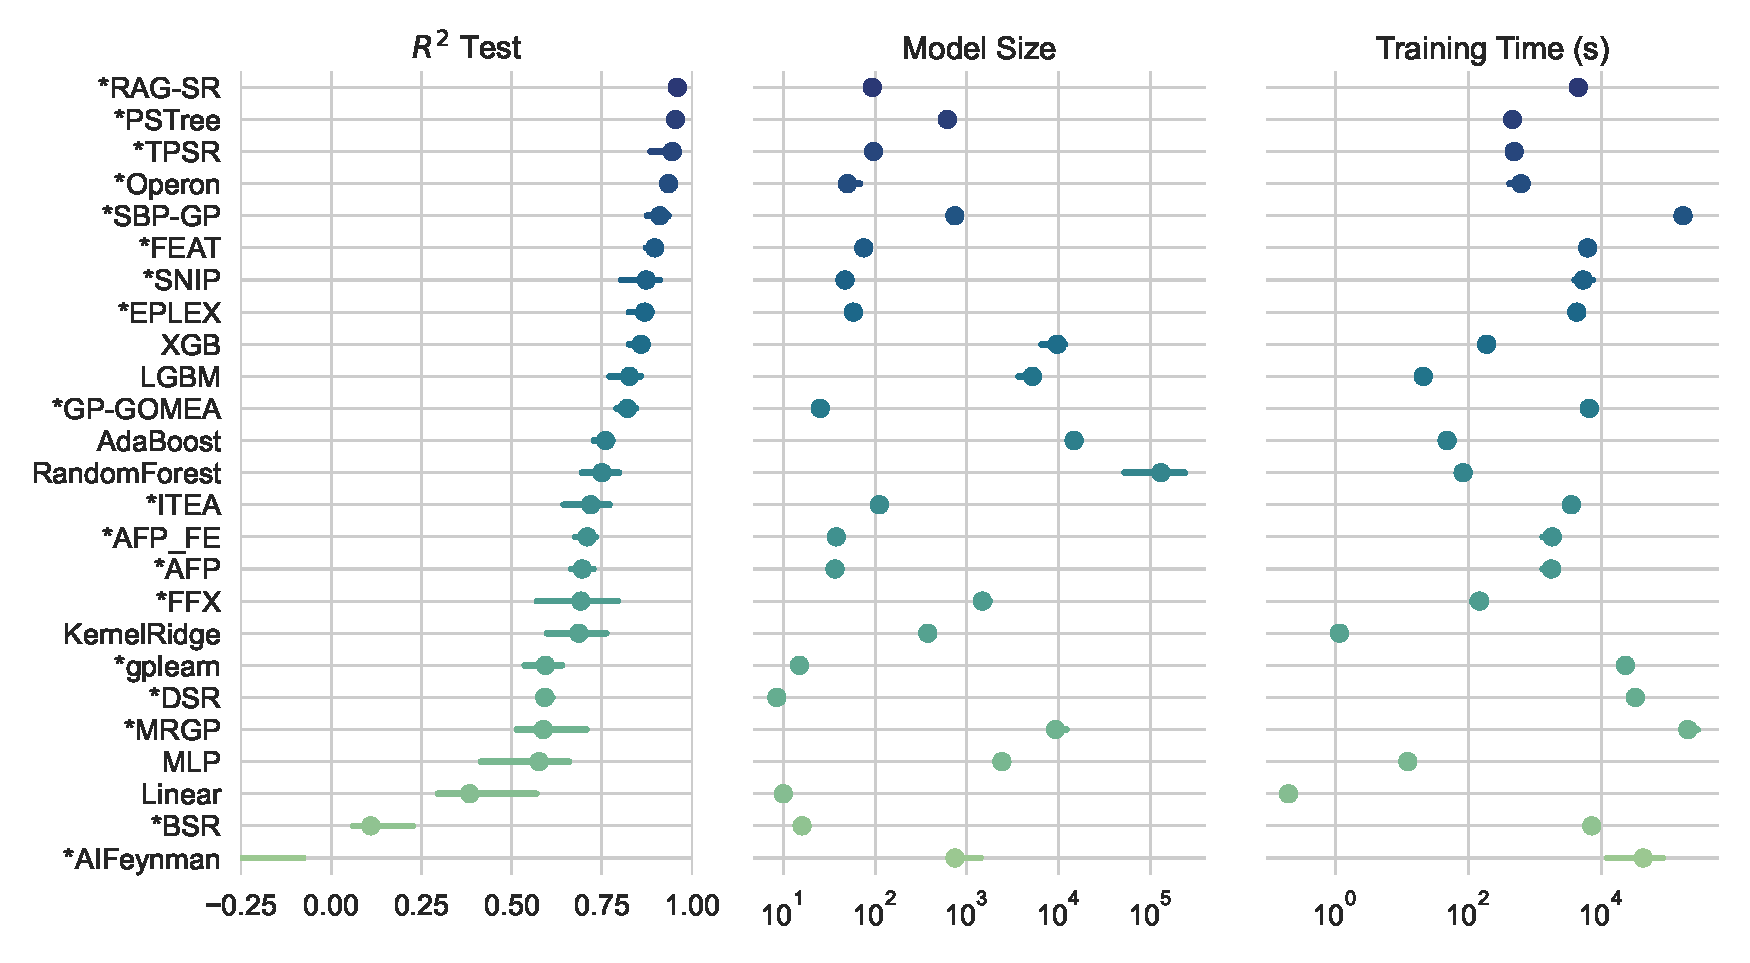
\includegraphics[width=\textwidth]{figs/pairgrid-pointplot_r2_test_model_size_training-time-(s).eps}
                \end{center}
            \end{column}

            \begin{column}{0.38\textwidth}
                \textbf{Observations:}
                \begin{itemize}
                    \item RAG-SR outperforms all 25 algorithms in $R^2$ scores
                    \item Produces models an order of magnitude smaller than SBP-GP
                    \item Training time comparable to FEAT
                    \item Best balance between accuracy, complexity, and efficiency
                \end{itemize}
            \end{column}
        \end{columns}
    \end{frame}

    \begin{frame}{Statistical Significance}
        \begin{columns}
            \begin{column}{0.48\textwidth}
                \begin{center}
                    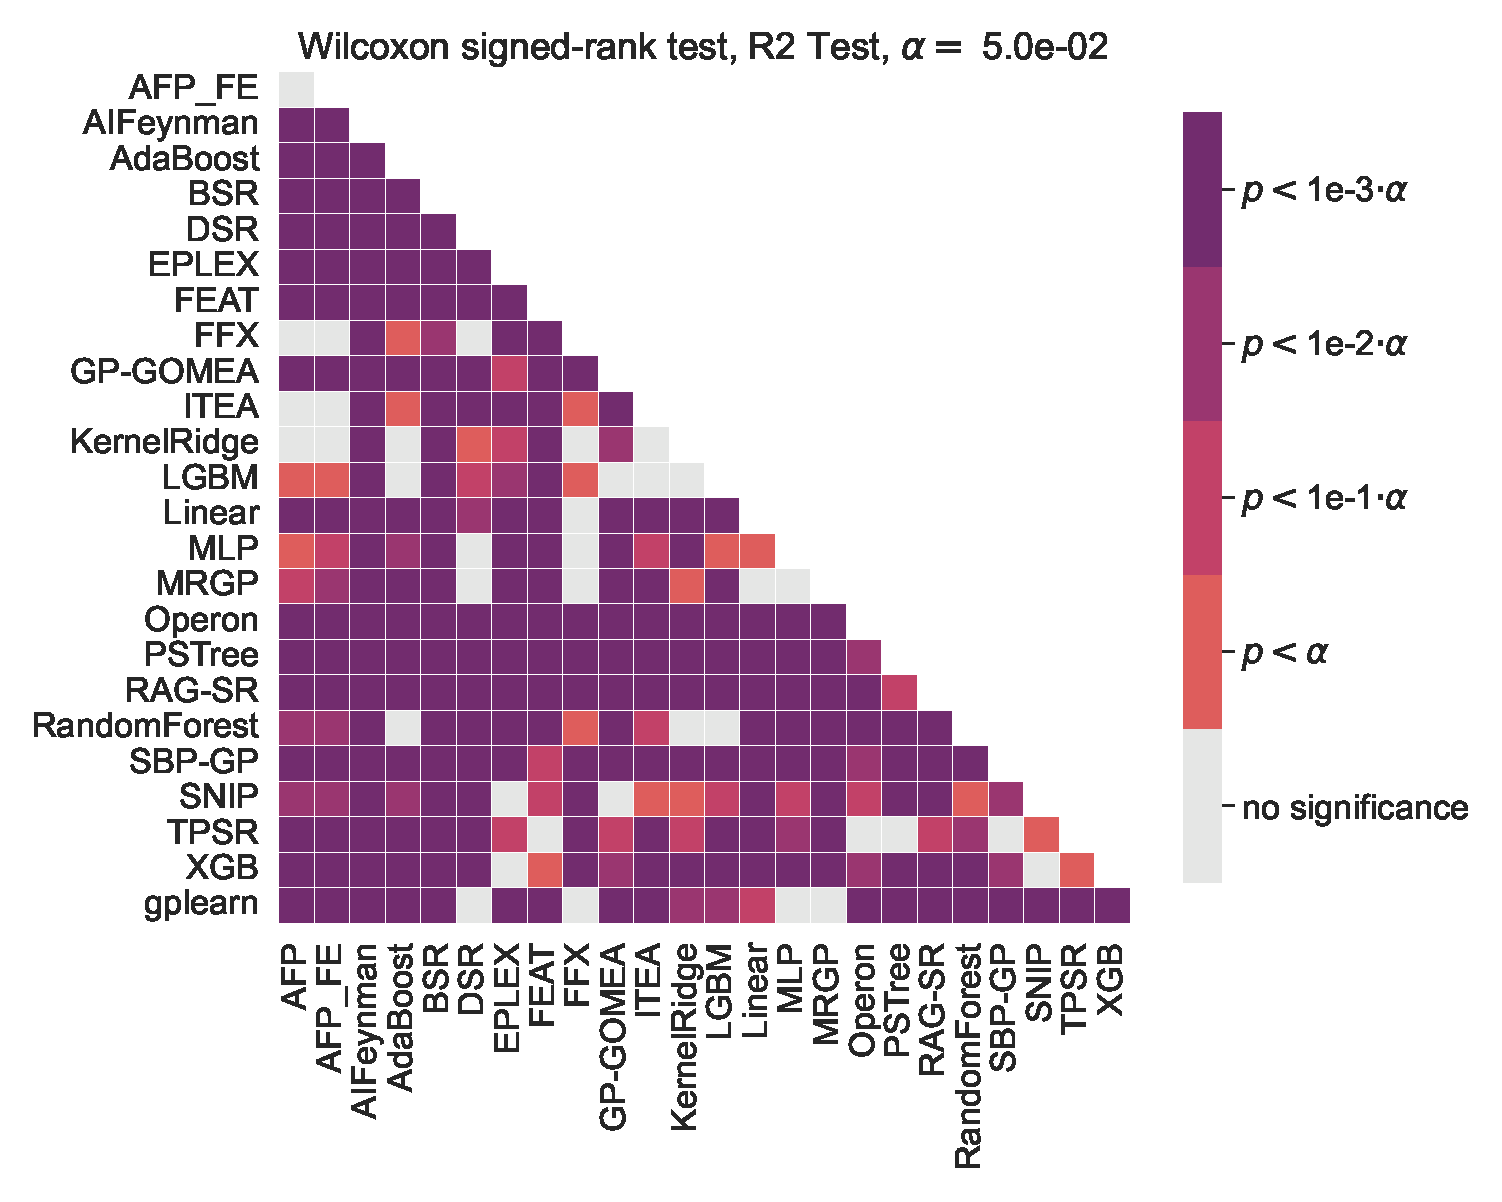
\includegraphics[width=\textwidth]{figs/Pairwise_comparison_of_R2_Test_on_black-box_problems.eps}
                \end{center}
            \end{column}

            \begin{column}{0.48\textwidth}
                \textbf{Observations:}
                \begin{itemize}
                    \item RAG-SR significantly outperforms all other methods
                    \item Improvement over TPSR confirms effectiveness of online learning vs. pre-training
                    \item Advantage over SBP-GP shows value of integrating a neural network component
                \end{itemize}
            \end{column}
        \end{columns}
    \end{frame}

    \begin{frame}{Pareto Front Analysis}
        \begin{columns}
            \begin{column}{0.48\textwidth}
                \begin{center}
                    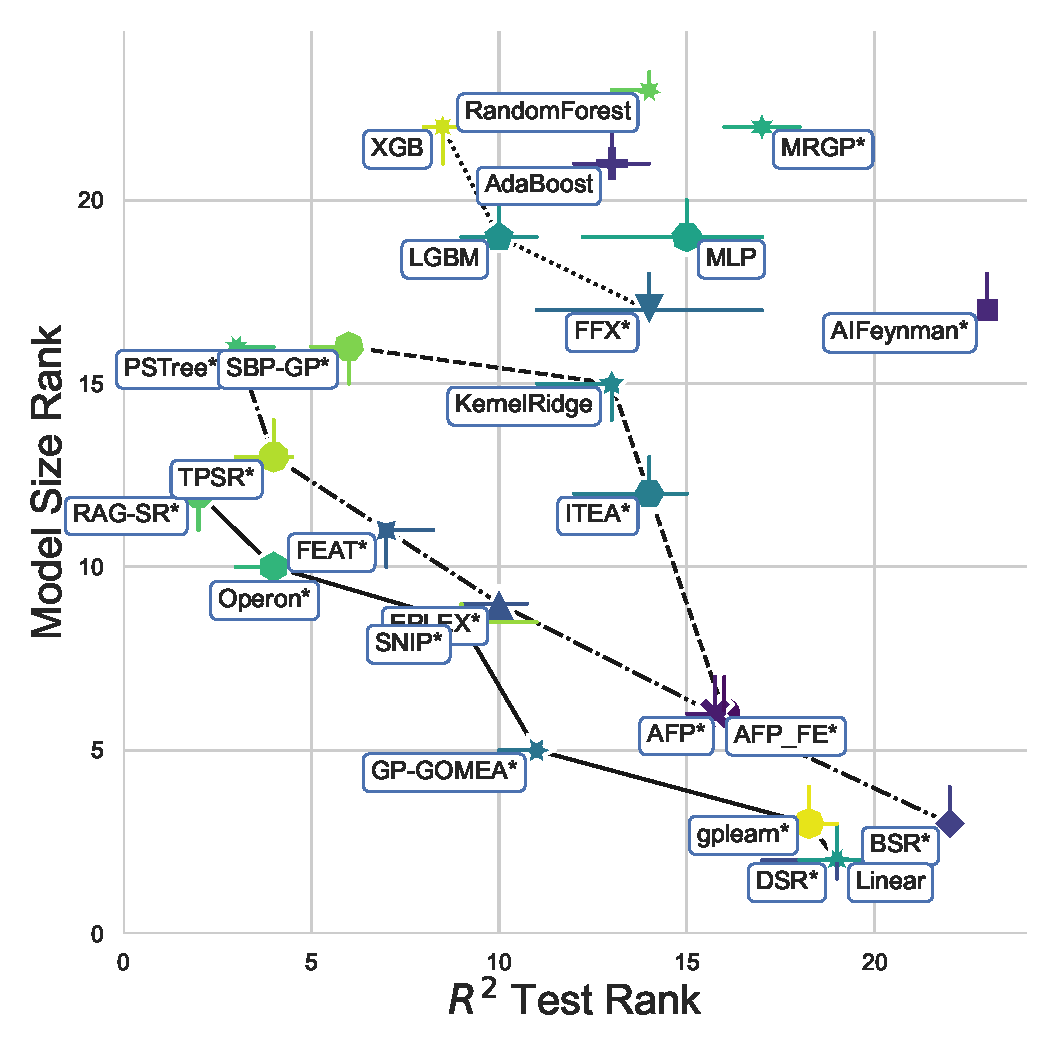
\includegraphics[width=\textwidth]{figs/pareto_plot_r2_test_rank_model_size_rank.eps}
                \end{center}
            \end{column}

            \begin{column}{0.48\textwidth}
                \textbf{Observations:}
                \begin{itemize}
                    \item RAG-SR appears on the first Pareto front
                    \item Excellent balance between accuracy and model complexity
                \end{itemize}
            \end{column}
        \end{columns}
    \end{frame}

    \begin{frame}{Feynman and Strogatz Results}
        \begin{center}
            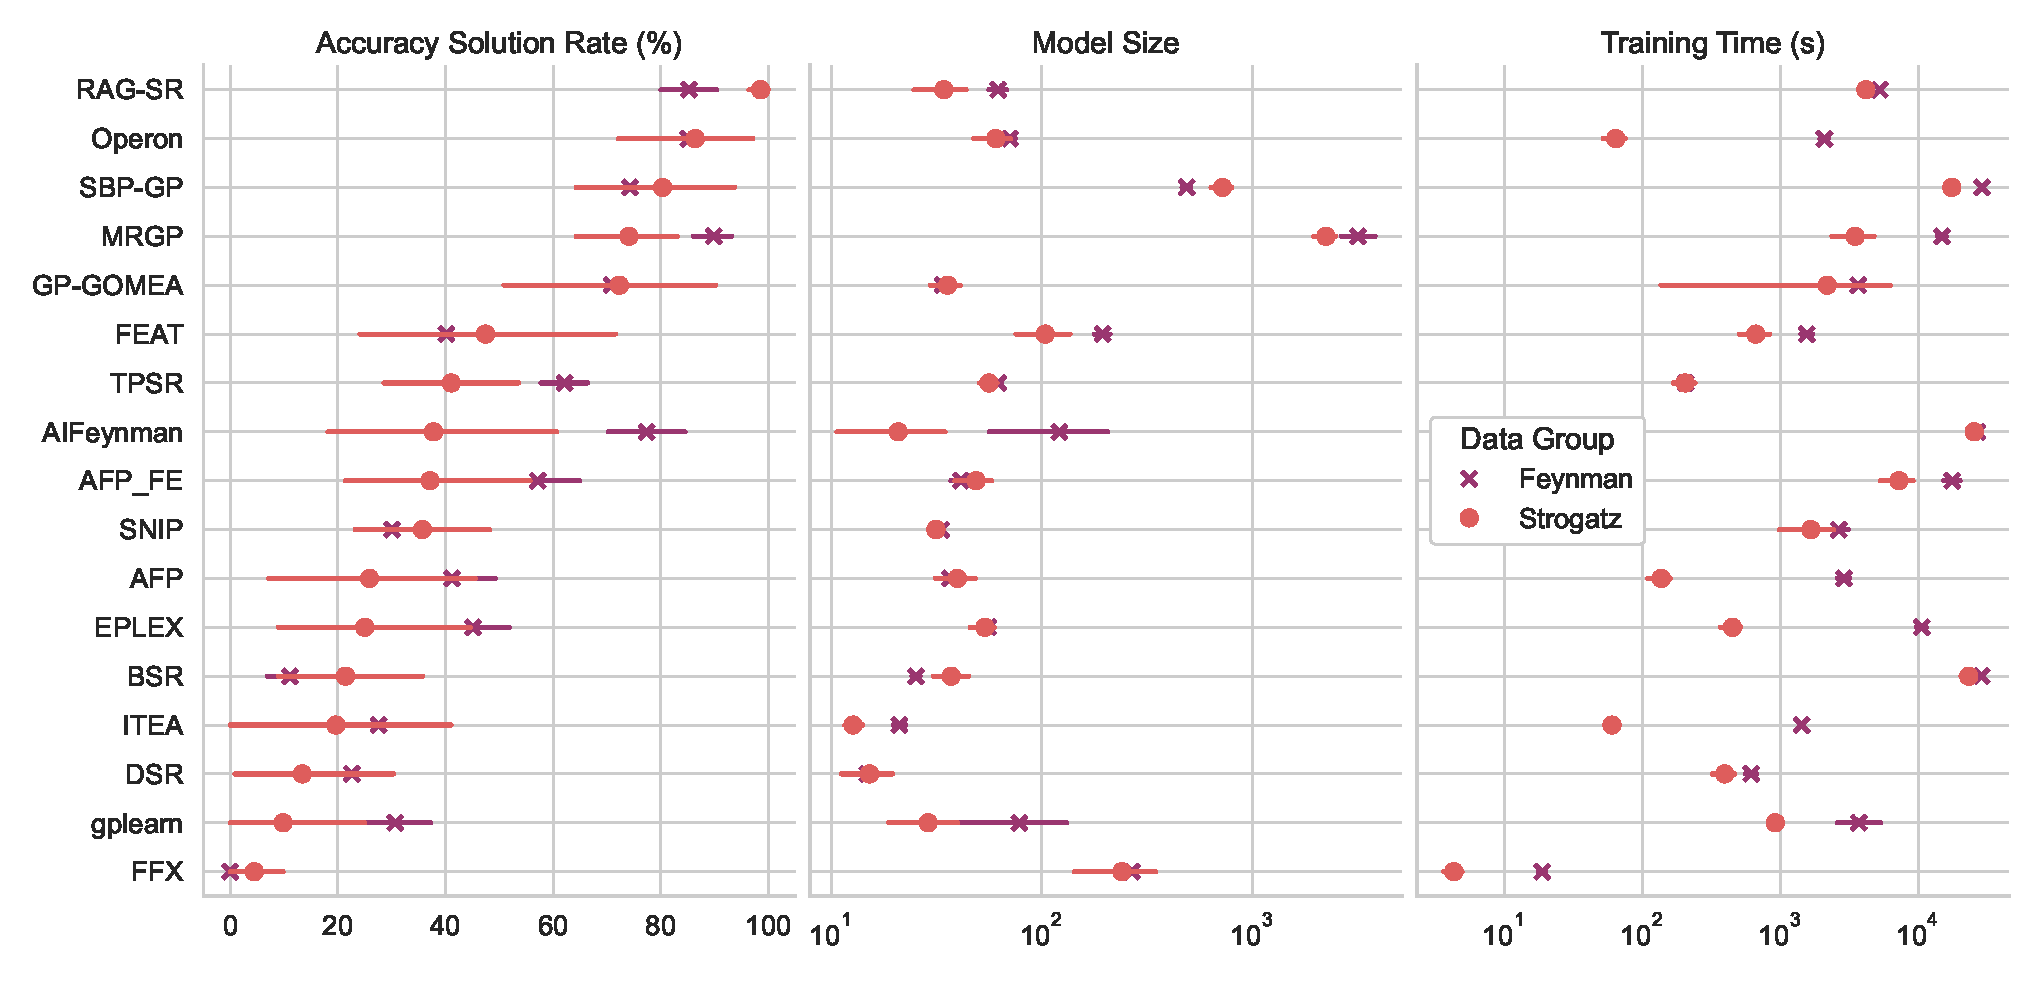
\includegraphics[width=0.8\textwidth]{figs/pairgrid_accuracy_solution_rate_(pct)_model_size_training-time-(s).eps}
        \end{center}

        \textbf{Observations:}
        \begin{itemize}
            \item Highest test $R^2$ scores on Strogatz datasets
            \item Second-best on Feynman datasets (after MRGP)
            \item MRGP models are an order of magnitude larger
            \item Significantly outperforms deep learning-based SR methods
        \end{itemize}
    \end{frame}


    \section{Conclusion}

    \begin{frame}{Conclusion}
        \textbf{Contributions:}
        \begin{itemize}
            \item Novel symbolic regression with retrieval-augmented neural semantic library
            \item Effective online learning approach without pre-training
            \item Retrieval augmentation that effectively mitigates hallucination
            \item Contrastive learning that considers semantic equivalence, improving effectiveness
            \item Data augmentation and double query that leverage sign-invariance, enhancing performance
        \end{itemize}

        \textbf{Future Directions:}
        \begin{itemize}
            \item Extending to noisy datasets with limited samples
            \item GPU acceleration for combining pre-training and online learning
        \end{itemize}
    \end{frame}

    \begin{frame}{Key Takeaway}
        \begin{center}
            \Large
            \alert{Key Innovation of RAG-SR:}

            \vspace{0.5cm}

            \begin{beamercolorbox}[rounded=true,shadow=true,sep=1em]{block body}
                Don't ask the NN to generate good improvements.\\
                \vspace{0.3cm}
                Instead, show examples of good improvements and say:\\
                'A good improvement is like this, now give a better one.'
            \end{beamercolorbox}
        \end{center}
    \end{frame}

    \begin{frame}{Thank You!}
        \begin{center}
            \Large{\textbf{Questions?}}

            \vspace{1cm}

            \normalsize
            Source Code: \url{https://github.com/hengzhe-zhang/RAG-SR}
        \end{center}
    \end{frame}
\end{document}